我們已經討論了程序的性能,還提到了高性能軟件。但這些代表了什麼呢?通常,我們知道高性能的程序比較快,但這並不意味著更快的程序總是有好的性能(兩個程序都可能有較差的性能)。

我們也提到了高效的程序,但是效率和高性能一樣嗎?雖然效率與性能有關,但並不相同。效率是指有效地利用資源,而不是浪費資源,而高效的程序會充分的利用計算硬件。

一方面,高效的程序不會讓可用的資源閒置。如果有需要完成的計算,而有處理器什麼都不做,那麼這個處理器應該正在等待執行的代碼。進一步的說,處理器中有許多計算資源,高效的程序可以同時利用盡可能多的資源。而高效的程序不會浪費資源去做不必要的工作,不會執行不需要的計算,不會浪費內存去存儲永遠不使用的數據,在不需要的情況下,不會通過網絡發送數據等。簡而言之,高效的程序不會讓可用的硬件閒置,也不會做不必要的工作。

另一方面,性能總是與一些指標相關。最常見的是“速度”,或程序運行的有多快。更嚴格地定義是\textit{吞吐量},即程序在給定時間內執行的計算量,或者說是計算特定結果所需的時間。然而,這並不是性能的唯一定義。

\subsubsubsection{1.3.1\hspace{0.2cm}性能——吞吐量}

考慮四個使用不同實現來計算相同結果的程序。下面是四個程序的運行時間(單位是相對的。實際數字並不重要,因為我們感興趣的是相對性能):

%\hspace*{\fill} \\ %插入空行
\begin{center}
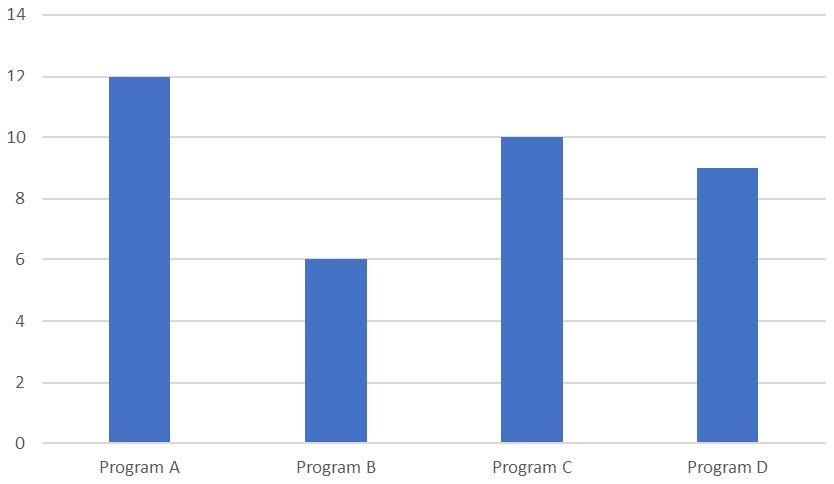
\includegraphics[width=0.8\textwidth]{content/1/chapter1/images/5.jpg}\\
圖1.5 - 同一算法,四種不同實現的運行時間(相對單位)
\end{center}

顯然,程序B的性能最高,比其他三個程序完成得早,計算同樣結果所需的時間是最慢程序的一半。通常,這將是我們選擇最佳實現所需的依據。

問題的背景很重要,我們忽略了這個程序是否是在電池供電的設備上運行的(比如手機),而且功耗指標也很重要。

\subsubsubsection{1.3.2\hspace{0.2cm}性能——功耗}

以下是四個程序在計算過程中所消耗的功率:

%\hspace*{\fill} \\ %插入空行
\begin{center}
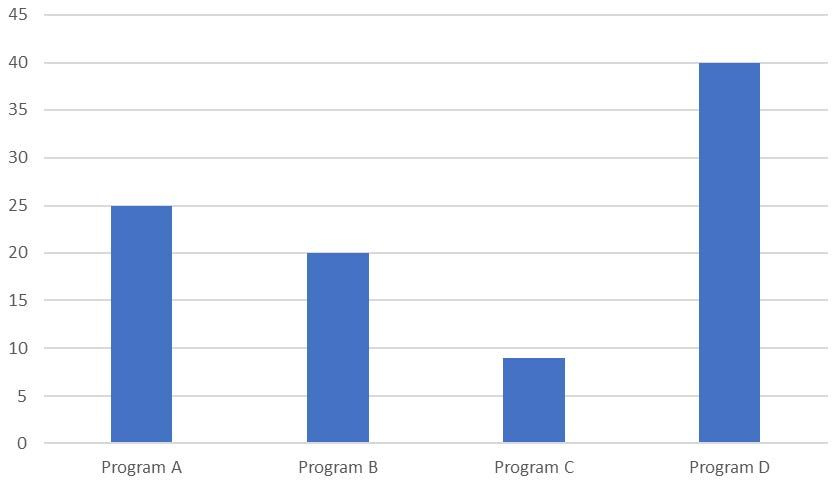
\includegraphics[width=0.8\textwidth]{content/1/chapter1/images/6.jpg}\\
圖1.6 - 同一算法,四種不同實現的功耗(相對單位)
\end{center}

雖然需要更長的時間才能得到結果,但是程序C總體上使用的功率更少。那麼,哪個程序的性能最好呢?

同樣,這是一個不瞭解完整背景的陷阱問題。程序不僅在移動設備上運行,而且執行實時計算,比如:用於音頻處理。這應該會讓結果更快地返回,對吧?不一定哦。

\subsubsubsection{1.3.3\hspace{0.2cm}性能——實時性}

實時程序必須時刻跟上它正在處理的事件,特別對於音頻處理器來說,必須跟上語音輸入。假設這個程序處理音頻的速度比人說話的速度快十倍,對我們來說這夠快了,所以不妨把注意力轉向功耗。

一方面,如果程序偶爾會落後於輸入,這樣一些聲音甚至文字就會消失。這說明實時或速度在一定程度上很重要,但必須以可知的方式進行交付。

當然,對此也有一個性能指標:尾部延遲。延遲是指數據準備好(語音記錄)和處理完成之間的延遲。前面的吞吐量反映了處理聲音的平均時間,如果對著手機說一個小時,那麼音頻處理器需要多長時間來完成所有計算?這種情況下,真正重要的是每個聲音的計算都需要按時完成。

在底層上,計算速度會波動:有時計算完成得快,有時時間會長。要是平均速度可以接受,那重點就在於是罕見的長延遲上了。

尾部延遲是作為延遲的特定百分位數來計算的,例如:如果$ t $有$95^{th}$個百分位的延遲,那麼95\%的所有計算花費的時間會比t少。指標本身是$95^{th}$個百分位時間$ t $與平均計算時間$ t_0 $的比率(經常表示為百分比,所以$95^{th}$個百分位的30\%延遲意味著$ t $比$ t_0 $大30\%):

%\hspace*{\fill} \\ %插入空行
\begin{center}
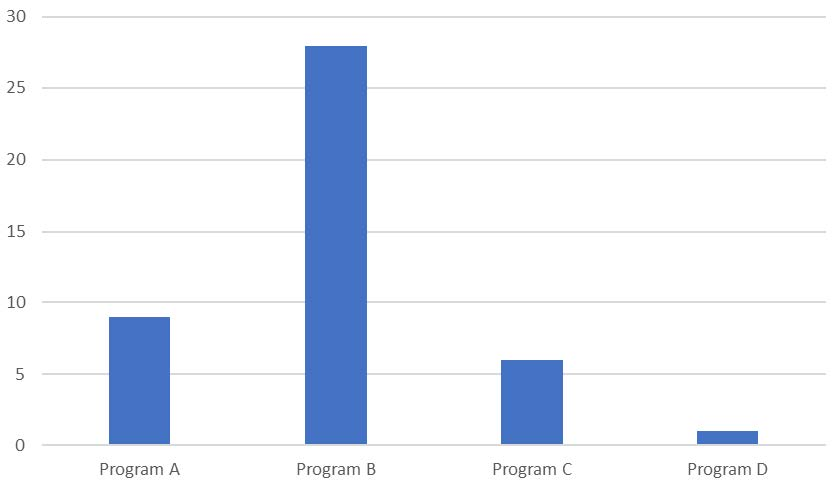
\includegraphics[width=0.9\textwidth]{content/1/chapter1/images/7.jpg}\\
圖1.7 - 95\%相同算法的四種不同實現的延遲(百分比)
\end{center}

平均下來程序B的計算結果比其他任何實現都快,它也提供了最不可預測的運行時間結果。而程序D的計算像發條一樣精確,每次做一個給定的計算幾乎花費相同的時間。我們已經觀察到,程序D的功耗是最差的。這很罕見,因為使程序更節能的技術,本質上是概率性的。大多數時候會加快計算速度,但也並不是每次都會這樣。

那麼,哪個程序的性能最好呢?答案肯定取決於程序,但即便如此,區別也可能並不明顯。

\subsubsubsection{1.3.4\hspace{0.2cm}性能——依賴上下文}

如果這是在大型數據中心中運行的仿真軟件,並且需要花費數天的時間來計算,那麼吞吐量就非常重要了。對於電池供電的設備,功耗通常是最重要的。在更復雜的環境中,比如實時音頻處理器,可能會是多個性能指標的組合。當然,平均運行時間也很重要,但只有當它“足夠快”時才重要。如果說話者沒有注意到延遲,處理的更快一點也什麼意義。需要注意尾部延遲,用戶的耐心會隨著漏詞,一點點的消耗殆盡。當延遲足夠好,通話質量則會受到其他因素的限制,那再關注這個點就沒什麼意義了,這時可以注意下能耗。

我們現在瞭解了,與效率不同,性能總是根據特定的指標來定義的,這些指標取決於應用程序和具體使用場景。對於某些指標來說,當其他指標出現時,就會出現“足夠好”的情況。效率反映了計算資源的利用情況,是實現良好性能的方法(可能是最常見的方法,但不是唯一的方法)。











